\documentclass[11pt,a4paper]{article}
\usepackage{ifpdf}
\usepackage[utf8]{inputenc}
\usepackage[francais]{babel}
\usepackage[T1]{fontenc}
\usepackage[nottoc, notlof, notlot]{tocbibind}
\usepackage[unicode=true,pdftex,colorlinks=true,linkcolor=black,urlcolor=black,citecolor=black]{hyperref}
\usepackage{natbib}
\usepackage{graphicx}

\parindent 0.8cm
%\setlength{\parskip}{0.5em plus 0.2em minus 0.2em}

\title{Projet Service : ALMA' Turn-keyWeek-End}
\author{Anthony \textsc{Caillaud} Manoël \textsc{Fortun}}
\date{\today}
\ifpdf
\pdfinfo {
/Author (Anthony Caillaud Manoël Fortun)
/Title (Projet Service : ALMA' Turn-keyWeek-End)
/Subject (Projet Service : ALMA' Turn-keyWeek-End)
/Keywords ()
/CreationDate (D:20100329212218)
}
\fi


\begin{document}

\maketitle


\clearpage
\tableofcontents
\clearpage
\section{Introduction}

Dans le cadre du module Service dans lequel nous avons étudié tous les
mécanismes et tous les éléments d'une architecture basée sur les services, nous
avons dû mettre en place une SOA complet. Ce SOA doit permettre à un utilisateur
de réserver plusieurs éléments pour un week-end pour deux personnes. Ces
éléments à réserver sont le voyage jusqu'à la destination, deux tickets pour
une manifestation, une chambre pour une nuit dans un hôtel et un diner dans un
restaurant. Afin d'obtenir une SOA fonctionnelle, nous avons d'abord mis en
place notre base de données et déterminé les tables nécessaires. Ensuite, nous
avons fixé les services nécessaires pour le bon déroulement de l'application, du
choix de l'utilisateur jusqu'aux différentes réservations. Une partie
importante de cette architecture sont les interfaces. L'une
d'entre-elle qui sera la façade de notre application pour l'utilisateur et
l'autre qui sera le back office permettant la gestion des entrées dans les
tables vous seront présentées. Enfin la génération du bon de réservation à
partir des données choisies par l'utilisateur à l'aide d'une transformation
XSLT permettra à celui-ci d'obtenir ce document en dans un fichier pdf.


\section{Définition de la base de données}
Pour cette architecture, nous avons utilisé une base de données comprenant les
différentes tables nécessaires au bon fonctionnement de l'application. Notre
base de données contient donc onze tables. 

Tout d'abord, il y cinq tables qui contiennent toutes les entrées représentant
les choix proposés à l'utilisateur. Ces tables sont les suivantes :\\

\begin{itemize}
  \item La table LOCALISATION qui permet de choisir un pays et une ville,
  \item La table TYPE MANIFESTATION qui permet de choisir le type de
  manifestation,
  \item La table MANIFESTATION qui permet de choisir une manifestation d'un
  certain type et qui a lieu dans le pays et la ville choisis,
  \item La table HOTEL qui permet de choisir un hôtel présent dans la ville
  choisie,
  \item La table RESTAURANT qui permet de choisir un restaurant présent dans la
  ville choisie.\\
\end{itemize}
 
Ensuite, cinq autres tables permettent l'enregistrement des différentes
réservations effectuées par l'utilisateur. Ces tables sont les suivantes :\\

\begin{itemize}
  \item La table VOYAGE qui enregistre la réservation du voyage entre la ville
  de départ et la ville d'arrivée,
  \item La table RESERVATION MANIF qui enregistre la réservation des deux tickets
  pour la manifestation choisie,
  \item La table RESERVATION HOTEL qui enregistre la réservation d'une chambre pour
  une nuit dans l'hôtel choisi,
  \item La table RESERVATION RESTAURANT qui enregistre la réservation d'un
  diner au restaurant,
  \item La table RESERVATION qui enregistre toutes les données concernant les
  réservations du week-end.\\
\end{itemize}

Enfin, la dernière table est la table CLIENT qui permet l'enregistrement du nom
et du prénom de l'utilisateur voulant effectuer ce week-end.


\section{Les différents services}
\subsection{La recherche des disponibilités}
\subsection{Les réservations}

\section{Les interfaces}
\subsection{Définition de l'interface}
\subsubsection{L'interface JSP}
\subsubsection{GoogleMaps}
\subsection{Le back office}

Pour ce projet nous devions aussi dévelloper une application dites de backoffice. Le role d'une application de ce type est de pouvoir administrer finement toutes les tables de la base de données, permettant de voir les enregistrement existant et d'en insérer de nouveau. 

Nous avions plusieurs piste pour le devellopement, nous avions étudié la possibilité de tout générer grâce à Symphony qui permet de générer des applis backoffice en php, seulement nous n'avons pas pu le mettre en place, et comme nous ne savions pas si nous aurions pu le déployer à la fac. Nous avons donc choisi de dévelloper notre application en java classique en swing comme le suggérait le sujet.

Develloper une tel application n'est pas spécialement compliqué, mais ne contient aucun aspects liés au module de service, aucune technologie vu durant le module n'a servit pour cette partie du projet.

Nous avons donc finalement develloper notre application en swing avec l'aide du framework Hibernate. 


\subsubsection{Architecture}

Avant de nous lancer dans le developpement de ce module du projet nous avons défini son architecture en fonction des outils utilisés, le schéma \ref{backoffice} 

\begin{figure}[h]
  		\centering
  		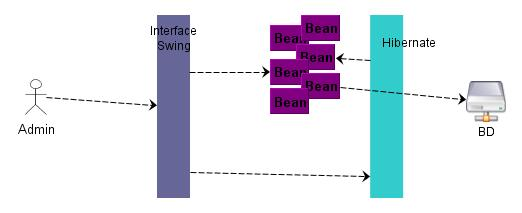
\includegraphics[height=14cm,width=15cm]{backoffice.jpg}
  		\caption{backoffice}
  		\label{Architecture du backoffice}
\end{figure}

Le diagramme \ref{backoffice} montre les interractions basiques entre tout les éléments, on voit l'utilisateur qui interragit avec l'interface en swing. L'interface qui interroge la couche hibernate, couche qui gére la liaison avec la base de donnée, couche qui renvoi des classes dites beans représentant les enregistrements dans la base. Cette architecture et l'utilsation de hibernate nous à permis de gérer la base de donnée directement en java sans avoir à écrire de SQL. 

Pour mieux comprendre cette architecture il faut quelques explications sur hibernate et la façon dont nous l'avons mis en oeuvre.

\subsubsection{hibernate}

Hibernate est un framework qui permet un mapping entre objet et base de données, de manière à ce que les tables et classes soient en relation et que les enregistrements des tables existent sous la forme d'instances de classe. De fait une modification sur une instance est répercuté sur la base de donnée de façon très simple, celà permet de facilement faire abstraction de la base et du langage associé.

Pour mettre en place ce framework dans notre module, nous nous sommes servit de netbean et des fonctions intégrée. Grâce au plugin intégré dans netbean nous avons pu générer de façon automatique les classes représentant les tables, ce qui nous fit gagner du temps, ces classes représentants les tables sont appellés Entity ou beans. La génération à simplement eut besoin de connaitre les identifiants de la BD et sa localisation, le reste à été automatique. Après nous avons du écrire les quelques méthodes qui permettent de récupérer les objets de la base de donnée et faire les actions dessus, comme la création, la modification et suppresion, ces fonctions sont contenu dans un objet nommé Session. Nous avons develloper ces fonctions sans écrire une seule ligne de SQL, le seul sql qui fut écrit le fut pour la création initiale de la base de données.

Une fois l'objet session défini ainsi que les beans, nous avons utilisé la bibliothèque swing pour les affichers et les modifier.

\subsubsection{Swing}



Utilisation de swing tout ça



tjable organiser les donnée
Interfacequi évolue
le moins possible de vue
faire simple.

\section{Génération du bon de réservation}
Une fois toute l'architecture mise en place et les réservations effectuées, il
ne restait plus qu'à produire un bon de réservation dans un fichier au format
pdf.
Pour cela, nous avons d'abord produit un fichier XML à partir de toutes les
données récupérées à partir du formulaire à l'aide de la librairie JDOM en
Java. Ensuite, pour aboutir à un fichier pdf, nous avons utilisé le formateur
Apache FOP(Formatting Objects Processor) qui permet d'en obtenir un à l'aide
d'un fichier XML et d'un fichier XSL-FO.


\section{Conclusion}

Utilisation de netbean pas particulièrement très agréable. 
Projet très ambitieux pour un projet de module avec trop d'aspect étranger au module 
Pas assez de temps
Une partie du projet sur lequel on ne peut avoir aucun support
prof de merde
gros connard


\end{document}
